\chapter{Operads and their algebras}

\section{Operads} \label{operad}

\begin{defn} Operads $O$ \end{defn}

\begin{namedexample}[(The symmetric operad)]
There is an operad $\mathrm{S}$ whose sets of operations $\mathrm{S}(n)$ for each $n \in \mathbb{N}$ are the underlying sets of the symmetric groups $\mathrm{S}_n$. The identity element of this \emph{symmetric operad} is the identity permutation of a single object, $e_1 \in \mathrm{S}_1$, and the operadic multiplication is defined in the following way:
\begin{itemize}
\item First, there exist maps $\otimes : \mathrm{S}_m \times \mathrm{S}_n \to \mathrm{S}_{m+n}$ called the \emph{direct sum} or \emph{block sum} of permutations. For any $\sigma \in \mathrm{S}_m$ and $\tau \in \mathrm{S}_n$, these are given by
\begin{eq*} (\sigma \otimes \tau)(i) \quad = \quad \begin{cases}
								\quad \sigma(i) & \quad 1 \le i \le m \\
								\quad \tau(i-m) +m & \quad m+1 \le i \le m+n
							\end{cases}
\end{eq*}
As the name suggests, this direct sum is usually denote by the symbol $\oplus$, but we will stick with $\otimes$ so that our notation here matches all of the other tensor products we will see throughout this paper. Also, notice that the value of these direct sums in general are determined by those specific cases where one of the inputs is an identity permutation:
\begin{eq*} \sigma \otimes \tau \quad = \quad (\sigma \otimes e_n) \cdot (e_m \otimes \tau) \quad = \quad (e_m \otimes \tau) \cdot (\sigma \otimes e_n) \end{eq*}
\item Next, we'll define functions $( \, \_ \, )_{(k_1, ..., k_n)} : \mathrm{S}_n \to \mathrm{S}_{k_1 + ... + k_n}$ for all $n, k_1, ..., k_n \in \mathbb{N}$. These will act by sending each $\sigma$ that permutes $n$ individual objects to a corresponding $\sigma_{(k_1, ..., k_n)}$ that permutes blocks of objects of size $k_1, ..., k_n$ in the same way. More concretely, if $k_1 + ... + k_{i-1} < j \le k_1 + ... + k_i$ then
\begin{eq*} \sigma_{(k_1, ..., k_n)}(j) \quad = \quad j - k_1 - ... - k_{i-1} + k_{\sigma^{-1}(1)} + ... + k_{\sigma^{-1}( \, \sigma(i) -1 \, )} \end{eq*}
\item Finally, the multiplication maps $\mu: \mathrm{S}_n \times \mathrm{S}_{k_1} \times ... \times \mathrm{S}_{k_n} \to \mathrm{S}_{k_1 + ... + k_n}$ are given by
\begin{eq*} \begin{array}{rll} 
			\mu(\sigma; \tau_1, ..., \tau_n) & := & \sigma_{(k_1, ..., k_n)} \cdot (\tau_1 \otimes ... \otimes \tau_n) \\
			& = & (\tau_{\sigma^{-1}(1)} \otimes ... \otimes \tau_{\sigma^{-1}(n)}) \cdot \sigma_{(k_1, ..., k_n)}
		\end{array}
\end{eq*}
In other words, the operadic multiplication of permutations comes from both permutating objects within distinct blocks and also permuting the blocks themselves.
\end{itemize}

If we decide to represent elements of the symmetric operad pictorially --- for example as strings which cross over another according to the appropriate permutation --- then both $\sigma \otimes \tau$ and $\sigma_{(k_1, ..., k_n)}$ have rather nice interpretations. The direct sum of two permutations is just the result of placing two permutations `next to' each other,
\begin{center} \begin{tabular}{ccccc}
			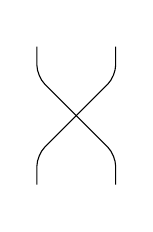
\begin{tikzpicture}[baseline]
				\node(x1) at (-0.5,1){};
				\node(y1) at (0.5,1){};	
				\node(y2) at (-0.5, -1){};
				\node(x2) at (0.5, -1){};
       				\draw[rounded corners](x1.south) to (-0.5,0.5) to (0.5,-0.5) to (x2.north);
				\draw[rounded corners](y1.south) to (0.5, 0.5) to (-0.5, -0.5) to (y2.north);		
			\end{tikzpicture} & \quad $\bigotimes$ \quad \quad &
			\begin{tikzpicture}[baseline]
				\node(x1) at (-0.5,1){};
				\node(y1) at (0.5,1){};	
				\node(x2) at (-0.5, -1){};
				\node(y2) at (0.5, -1){};
				\draw[rounded corners](x1.south) to (x2.north);	
       				\draw[rounded corners](y1.south) to (y2.north);	
			\end{tikzpicture} & \quad $=$ \quad \quad &
			\begin{tikzpicture}[baseline]
				\node(x1) at (-1.5,1){};	
				\node(y1) at (-0.5,1){};
				\node(y2) at (-1.5, -1){};
				\node(x2) at (-0.5, -1){};
				\node(x'1) at (0.5,1){};
				\node(y'1) at (1.5,1){};
				\node(x'2) at (0.5, -1){};
				\node(y'2) at (1.5, -1){};
       				\draw[rounded corners](x1.south) to (-1.5,0.5) to (-0.5,-0.5) to (x2.north);	
				\draw[rounded corners](y1.south) to (-0.5, 0.5) to (-1.5, -0.5) to (y2.north);
				\draw[rounded corners](x'1.south) to (x'2.north);	
       				\draw[rounded corners](y'1.south) to (y'2.north);	
			\end{tikzpicture} \\
			$\sigma$ & & $\tau$ & & $\sigma \otimes \tau$
\end{tabular} \end{center}
and block permutations are given by expanding string into some number of parallel strings,
\begin{center} \begin{tabular}{ccc}
			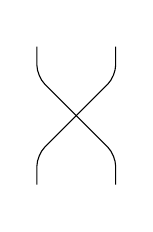
\begin{tikzpicture}[baseline]
				\node(x1) at (-0.5,1){};
				\node(y1) at (0.5,1){};	
				\node(y2) at (-0.5, -1){};
				\node(x2) at (0.5, -1){};
       				\draw[rounded corners](x1.south) to (-0.5,0.5) to (0.5,-0.5) to (x2.north);
				\draw[rounded corners](y1.south) to (0.5, 0.5) to (-0.5, -0.5) to (y2.north);		
			\end{tikzpicture} & \quad $\mapsto$ \quad \quad &
			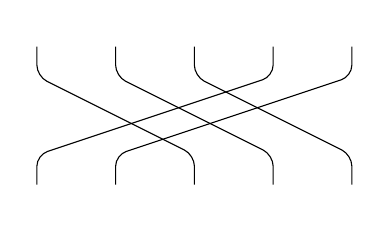
\begin{tikzpicture}[baseline]
				\node(x1) at (-2,1){};
				\node(x'1) at (-1,1){};
				\node(x''1) at (0,1){};
				\node(y1) at (1,1){};	
				\node(y'1) at (2,1){};
				\node(y2) at (-2, -1){};
				\node(y'2) at (-1, -1){};
				\node(x2) at (0, -1){};
				\node(x'2) at (1, -1){};
				\node(x''2) at (2, -1){};
       				\draw[rounded corners](x1.south) to (-2,0.5) to (0,-0.5) to (x2.north);
       				\draw[rounded corners](x'1.south) to (-1,0.5) to (1,-0.5) to (x'2.north);
       				\draw[rounded corners](x''1.south) to (0,0.5) to (2,-0.5) to (x''2.north);
				\draw[rounded corners](y1.south) to (1, 0.5) to (-2, -0.5) to (y2.north);
				\draw[rounded corners](y'1.south) to (2, 0.5) to (-1, -0.5) to (y'2.north);	
			\end{tikzpicture} \\
			$\sigma$ & & $\sigma_{(3, 2)}$
\end{tabular} \end{center}
With a little work, we can actually replace the functions $( \, \_ \, )_{(k_1, ..., k_n)}$ with an explicit combination of group multiplication and tensor product. This is due to basic fact about the symmetric groups $\mathrm{S}_n$, which is that they possess a presentation in terms of the \emph{elementary transpositions} $(i \,\,\,  i+1)$.

\begin{lem} \label{sympres} The group $\mathrm{S}_n$ is generated by the permutations $(1 \, 2), ..., (n-1 \, \, \, n)$, subject to the relations
\begin{eq*} \begin{array}{rclll}
			(i \, \, \, i+1)^2 & = & e & & \\
			(i-1 \, \, \, i)(i \, \, \, i+1)(i-1 \, \, \, i) & = & (i \, \, \, i+1)(i-1 \, \, \, i)(i \, \, \, i+1) & & \\
			(i \, \, \, i+1)(j \, \, \, j+1) & = & (j \, \, \, j+1)(i \, \, \, i+1), & & i+1 < j
		\end{array}
\end{eq*}
\end{lem}

Thus if $\sigma \in \mathrm{S}_n$ is a permutation with a decomposition $\sigma = \sigma_m \cdot ... \cdot \sigma_1 $ in terms of elementary transpositons $\sigma_i \in \mathrm{S}_n$, we can break down the block permutation $\sigma_{(k_1, ..., k_n)}$ into the $m$ `elementary block transpositions' $(\sigma_i)_{(k_1, ..., k_n)}$:
\begin{eq*} \begin{array}{rll}
			\sigma_{(k_1, ..., k_n)}(j) & = & j - k_1 - ... - k_{i-1} + k_{\sigma^{-1}(1)} + ... + k_{\sigma^{-1}( \, \sigma(i) -1 \, )} \\
			& = & j - k_1 - ... - k_{i-1} \\
			& & + \, k_{\sigma_1^{-1}(1)} + ... + k_{\sigma_1^{-1}( \, \sigma_1(i) -1 \, )} \\
			& & -  \, k_{\sigma_1^{-1}(1)} - ... - k_{\sigma_1^{-1}( \, \sigma_1(i) -1 \, )} \\
			& & + \, k_{(\sigma_2 \sigma_1)^{-1}(1)} + ... + k_{(\sigma_2 \sigma_1)^{-1}( \, \sigma_2\sigma_1(i) -1 \, )} \\
			& & \vdots \\
			& & - \,  k_{(\sigma_{m-1}...\sigma_1^{-1}(1)} - ... - k_{(\sigma_{m-1}...\sigma_1)^{-1}( \, \sigma_{m-1}...\sigma_1(i) - 1 \, )} \\
			& & + \, k_{(\sigma_m...\sigma_1)^{-1}(1)} + ... + k_{(\sigma_m...\sigma_1)^{-1}( \, \sigma_m...\sigma_1(i) - 1 \, )} \\
			& = & \big( \, (\sigma_m)_{(k_1, ..., k_n)} \cdot ... \cdot (\sigma_1)_{(k_1, ..., k_n)} \, \big)(j)
		\end{array}
\end{eq*}
However, since elementary transpositions only really permute two objects, they can be written as a block sum in the operad $\mathrm{S}$ involving the sole transposition of $\mathrm{S}_2$, plus some number of identity permutations.
\begin{eq*} (i \, \, \, i+1) \quad = \quad e_{i-1} \otimes (1 \, 2) \otimes e_{n-i-1} \end{eq*}
This means that the elementary block transpositions are
\begin{eq*} \begin{array}{rll}
			(i \, \, \,  i+1)_{(k_1, ..., k_n)} & = & \quad (e_{i-1} \otimes (1 \, 2) \otimes e_{n-i-1})_{(k_1, ..., k_n)} \\
			& = & e_{k_1 + ... k_{i-1}} \otimes (1 \, 2)_{(k_i, k_{i+1})} \otimes e_{k_{i+1} + ... k_n}
		\end{array}
\end{eq*}
So all we need to know to fully understand the functions $( \, \_ \, )_{(k_1, ..., k_n)}$ are the values they take on the transposition $(1 \, 2)$. These can be defined recursively, via
\begin{eq*} \begin{array}{rclcrcl}
			(1 \, 2)_{(0, n)} & = & e_n, & \quad \quad & (1 \, 2)_{(m+m', n)} & = & \big( \, (1 \, 2)_{(m, n)} \otimes e_{m'} \, \big) \cdot \big( \, e_m \otimes (1 \, 2)_{(m', n)} \, \big) \\
			(1 \, 2)_{(m, 0)} & = & e_m, & \quad \quad & (1 \, 2)_{(m, n+n')} & = & \big( \, e_n \otimes (1 \, 2)_{(m, n')} \, \big) \cdot \big( \, (1 \, 2)_{(m, n)} \otimes e_{n'} \, \big) 			
		\end{array}
\end{eq*}
which all follow from the definition of $( \, \_ \, )_{(k_1, ..., k_n)}$. Therefore all $\sigma_{(k_1, ..., k_n)}$ and hence all $\mu(\sigma; \tau_1, ..., \tau_n)$ can be expressed in terms of group multiplication $\cdot$ and direct sum $\otimes$, and the elementary permutations which constitute $\sigma, \tau_1, ..., \tau_n$.
\end{namedexample}

\begin{namedexample}[(The braid operad)]\label{braidop}
The \emph{braid groups} $B_n$ are the family of groups that result from taking the symmetric groups and removing the requirement that everything needs to be self-inverse. That is, the group $B_n$ has a presentation on some \emph{elementary braids} $b_1, ..., b_{n-1}$, given by the relations
\begin{eq*} b_i b_{i+1} b_i \, = \, b_{i+1} b_i b_{i+1}, \quad \quad \quad \quad \quad b_i b_j \, = \, b_j b_i, \quad i+1 < j \end{eq*}
As might be expected, the underlying sets of these groups also form an operad, known as the \emph{braid operad} $B$, and they do so in a way directly analagous to the operad $\mathrm{S}$. That is, the identity element of $B$ is $e_1 \in \mathrm{B}_1$, and the operadic multiplication is constructed as follows:
\begin{itemize}
\item Tensor products $\otimes : B_m \times B_n \to B_{m+n}$ are determined by setting 
\begin{eq*} x \otimes y \quad = \quad (x \otimes e_n) \cdot (e_m \otimes y) \quad = \quad (e_m \otimes x) \cdot (y \otimes e_n) \end{eq*}
for all $x \in B_m$, $y \in B_n$, and also
\begin{eq*} b_i \quad = \quad e_{i-1} \otimes b \otimes e_{n-i-1} \end{eq*}
for any elementary braid $b_i \in B_n$, where $b$ is the only elementary braid in $B_2$.
\item The functions $( \, \_ \, )_{(k_1, ..., k_n)} : B_n \to B_{k_1 + ... + k_n}$ are first defined recursively on the elementary braid $b \in B_2$ by
\begin{eq*} \begin{array}{rclcrcl}
			b_{(0, n)} & = & e_n, & \quad \quad & b_{(m+m', n)} & = & (b_{(m, n)} \otimes e_{m'}) \cdot (e_m \otimes b_{(m', n)}) \\
			b_{(m, 0)} & = & e_m, & \quad \quad & b_{(m, n+n')} & = & (e_n \otimes b_{(m, n')}) \cdot (b_{(m, n)} \otimes e_{n'}) 			
		\end{array}
\end{eq*}
then on arbitrary elementary braids $b_i \in B_n$ via
\begin{eq*} (b_i)_{(k_1, ..., k_n)} \quad = \quad e_{k_1 + ... k_{i-1}} \otimes b_{(k_i, k_{i+1})} \otimes e_{k_{i+1} + ... k_n} \end{eq*}
and finally on all elements of the braid groups by using their presentation in terms of the $b_i$,
\begin{eq*} \begin{array}{rll}
			x & = & b_{i_m} \cdot ... \cdot b_{i_1} \\
			\implies \quad x_{(k_1, ..., k_n)} & = & (b_{i_m})_{(k_1, ..., k_n)} \cdot ... \cdot (b_{i_1})_{(k_1, ..., k_n)} 
		\end{array}
\end{eq*}
\item Then as in the symmetric case, the multiplication maps $\mu: B_n \times B_{k_1} \times ... \times B_{k_n} \to B_{k_1 + ... + k_n}$ are just
\begin{eq*} \mu(x; y_1, ..., y_n) \quad := \quad x_{(k_1, ..., k_n)} \cdot (y_1 \otimes ... \otimes y_n) \end{eq*}
\end{itemize}

These operations are exactly what they need to be in order for them to possess the same pictorial representations as the operations in $\mathrm{S}$, but with actual braids replacing simple crossings. That is, the tensor product $x \otimes y$ is the braids $x$ and $y$ laid side-by-side,
\begin{center} \begin{tabular}{ccccc}
			\begin{tikzpicture}[baseline]
				\node(x1) at (-0.5,1){};
				\node(y1) at (0.5,1){};	
				\node(y2) at (-0.5, -1){};
				\node(x2) at (0.5, -1){};
				\node(b) at (0,0)[circle,fill=white]{};
       				\draw[rounded corners](x1.south) to (-0.5,0.5) to (0.5,-0.5) to (x2.north);
				\begin{pgfonlayer}{bg}
				\draw[rounded corners](y1.south) to (0.5, 0.5) to (-0.5, -0.5) to (y2.north);
    				\end{pgfonlayer}	
			\end{tikzpicture} & \quad $\bigotimes$ \quad \quad &
			\begin{tikzpicture}[baseline]
				\node(x1) at (-0.5,1){};
				\node(y1) at (0.5,1){};	
				\node(x2) at (-0.5, -1){};
				\node(y2) at (0.5, -1){};
				\draw[rounded corners](x1.south) to (x2.north);	
       				\draw[rounded corners](y1.south) to (y2.north);	
			\end{tikzpicture} & \quad $=$ \quad \quad &
			\begin{tikzpicture}[baseline]
				\node(x1) at (-1.5,1){};	
				\node(y1) at (-0.5,1){};
				\node(y2) at (-1.5, -1){};
				\node(x2) at (-0.5, -1){};
				\node(b) at (-1,0)[circle,fill=white]{};
				\node(x'1) at (0.5,1){};
				\node(y'1) at (1.5,1){};
				\node(x'2) at (0.5, -1){};
				\node(y'2) at (1.5, -1){};
       				\draw[rounded corners](x1.south) to (-1.5,0.5) to (-0.5,-0.5) to (x2.north);	
				\begin{pgfonlayer}{bg}
				\draw[rounded corners](y1.south) to (-0.5, 0.5) to (-1.5, -0.5) to (y2.north);
    				\end{pgfonlayer}
				\draw[rounded corners](x'1.south) to (x'2.north);	
       				\draw[rounded corners](y'1.south) to (y'2.north);	
			\end{tikzpicture} \\
			$x$ & & $y$ & & $x \otimes y$
\end{tabular} \end{center}
and the `block braids' are multiple strings braided together in parallel,
\begin{center} \begin{tabular}{ccc}
			\begin{tikzpicture}[baseline]
				\node(x1) at (-0.5,1){};
				\node(y1) at (0.5,1){};	
				\node(y2) at (-0.5, -1){};
				\node(x2) at (0.5, -1){};
				\node(b) at (0,0)[circle,fill=white]{};
       				\draw[rounded corners](x1.south) to (-0.5,0.5) to (0.5,-0.5) to (x2.north);
				\begin{pgfonlayer}{bg}
				\draw[rounded corners](y1.south) to (0.5, 0.5) to (-0.5, -0.5) to (y2.north);
    				\end{pgfonlayer}		
			\end{tikzpicture} & \quad $\mapsto$ \quad \quad &
			\begin{tikzpicture}[baseline]
				\node(x1) at (-2,1){};
				\node(x'1) at (-1,1){};
				\node(x''1) at (0,1){};
				\node(y1) at (1,1){};	
				\node(y'1) at (2,1){};
				\node(y2) at (-2, -1){};
				\node(y'2) at (-1, -1){};
				\node(x2) at (0, -1){};
				\node(x'2) at (1, -1){};
				\node(x''2) at (2, -1){};
				\node(b1) at (-0.8,-0.1)[circle,fill=white]{};
				\node(b2) at (-0.2,0.1)[circle,fill=white]{};
				\node(b3) at (0.4,0.3)[circle,fill=white]{};
				\node(b4) at (-0.4,-0.3)[circle,fill=white]{};
				\node(b5) at (0.2,-0.1)[circle,fill=white]{};
				\node(b6) at (0.8,0.1)[circle,fill=white]{};
       				\draw[rounded corners](x1.south) to (-2,0.5) to (0,-0.5) to (x2.north);
       				\draw[rounded corners](x'1.south) to (-1,0.5) to (1,-0.5) to (x'2.north);
       				\draw[rounded corners](x''1.south) to (0,0.5) to (2,-0.5) to (x''2.north);
				\begin{pgfonlayer}{bg}
				\draw[rounded corners](y1.south) to (1, 0.5) to (-2, -0.5) to (y2.north);
				\draw[rounded corners](y'1.south) to (2, 0.5) to (-1, -0.5) to (y'2.north);
    				\end{pgfonlayer}	
			\end{tikzpicture} \\
			$x$ & & $x_{(3, 2)}$
\end{tabular} \end{center}
\end{namedexample}

\begin{defn} Operads maps \end{defn}

\cite{ogge} \cite{groupop}

\begin{defn}\label{actop} Action operads $G$, maps, $\mathrm{AOp}$ \end{defn}

There are a couple of operads which trivially have the structure of an action operads. 

First there is the \emph{terminal operad} $\mathrm{T}$, which has a single operation for each arity, so that $\mathrm{T}(n) = \{ e_n \}$. Each of these sets can be seen as the trivial group, and it follows from this that the $\pi^{\mathrm{T}} : \mathrm{T}(n) \to \mathrm{S}_n$ must be the respective zero maps, the terminal homomorphisms in the category of groups. The action operad condition is then
\begin{eq*} \mu(e_n; e_{k_1}, ..., e_{k_n}) \cdot \mu(e_n; e_{k_1}, ..., e_{k_n}) \quad = \quad \mu(e_n; e_{k_1}, ..., e_{k_n}) \end{eq*}
which is really just
\begin{eq*} e_{k_1 + ... + k_n} \cdot e_{k_1 + ... + k_n} \, = \, e_{k_1 + ... + k_n} \end{eq*}
and hence is trivially true. As its name suggests, the terminal operad is the terminal object in the category of operads, but it is also the \emph{initial} object in the category of action operads. This is because for any other $G$ in $\mathrm{AOp}$ the zero homomorphisms $\mathrm{T}(n) \to G(n)$ define the unique map of operads $f: \mathrm{T} \to G$.

On the other hand, it is the symmetric operad $\mathrm{S}$ itself that functions as the terminal object in $\mathrm{AOp}$. Its action operad structure is just given by the standard group multiplications on the $\mathrm{S}_n$, with the identity maps $\mathrm{id}_{\mathrm{S}_n} : \mathrm{S}_n \to \mathrm{S}_n$ functioning as its $\pi_n$. To see terminality, notice that for any other action operad $G$ a valid morphism $f: G \to \mathrm{S}$ in $\mathrm{AOp}$ must obey
\begin{eq*} \pi^{\mathrm{S}} \circ f \, = \, \pi^{G} \quad \implies \quad f \, = \, \pi^{G} \end{eq*}
Thus there only one map of action operads $G \to \mathrm{S}$, which is the very underlying permutation structure used to define $G$.

There are more interesting examples of action operads we can look at though. For instance, we know that the braid groups $B_n$ have the same presentation as the symmetric groups, except without the relations $b_i^2 = e$. Thus if we take their quotients by these relations we will obtain a sequence of homomorphisms $B_n \to \mathrm{S}_n$, each sending $b_i \mapsto (i \, \, \, i+1)$. This provides a natural way to describe the underlying permutation of any braid, and indeed choosing these maps to form $\pi^B$ gives a valid way of seeing the braid operad as an action operad. Another example can also be built with the so-called ribbon braid groups.

\begin{defn} For each $n \in \mathbb{N}$, the \emph{ribbon braid group} $RB_n$ is the group whose presentation is the same as that of the braid group $B_n$, except with the addition of $n$ new generators $t_1, ..., t_n$, known as the \emph{twists}. These twists all commute with one other, and also commute with all braids except in the following cases:
\begin{eq*} b_i \cdot t_i \quad = \quad t_{i+1} \cdot b_i, \quad \quad \quad \quad \quad b_i \cdot t_{i+1} \quad = \quad t_i \cdot b_i \end{eq*}
The \emph{ribbon braid operad} $RB$ is then the operad made up of these groups in a way that extends the definition of the braid operad. In other words, the identity is still $e_1 \in RB_1$, and the operadic multiplication is built up in stages in exactly the same ways as in \cref{braidop}, but with some additional rules for dealing with twists. For the tensor product, we have that for any twist $t_i \in RB_n$,
\begin{eq*} t_i \quad = \quad e_{i-1} \otimes t \otimes e_{n-i} \end{eq*}
where $t$ is the sole twist in $RB_1$, and for the `block twists' $t_{(m)}$ we again work recursively:
\begin{eq*} t_{(0)} \, = \, e_n, \quad \quad \quad t_{(m+m')} \quad = \quad (t_{(m)} \otimes t_{(m')}) \cdot b_{(m', m)} \cdot b_{(m, m')} \end{eq*}
\end{defn}

Much as the symmetric groups can be represented by crossings of a collection of strings, and the braid groups by braidings of strings, the ribbon braid groups deal with the ways that one can braid together several flat ribbons, including the ability to twist a ribbon about its own axis by 360 degrees.
\begin{center} \begin{tabular}{ccc}
			\begin{tikzpicture}[baseline]
				\node(xl1) at (-0.7,1){};
				\node(xr1) at (-0.3,1){};
				\node(yl1) at (0.3,1){};
				\node(yr1) at (0.7,1){};
				\node(yl2) at (-0.7, -1){};
				\node(yr2) at (-0.3, -1){};
				\node(xl2) at (0.3, -1){};
				\node(xr2) at (0.7, -1){};
				\node(b) at (0,0)[circle,fill=white, minimum size=0.5cm]{};
       				\draw[rounded corners](xl1.north) to (-0.7,0.5) to (0.3,-0.5) to (xl2.south);
       				\draw[rounded corners](xr1.north) to (-0.3,0.5) to (0.7,-0.5) to (xr2.south);
				\begin{pgfonlayer}{bg}
				\draw[rounded corners](yl1.north) to (0.3, 0.5) to (-0.7, -0.5) to (yl2.south);
				\draw[rounded corners](yr1.north) to (0.7, 0.5) to (-0.3, -0.5) to (yr2.south);
    				\end{pgfonlayer}
				\draw(xl1.north) to (xr1.north);
				\draw(xl2.south) to (xr2.south);
				\draw(yl1.north) to (yr1.north);
				\draw(yl2.south) to (yr2.south);
			\end{tikzpicture} & \quad \quad \quad \quad \quad \quad \quad &
			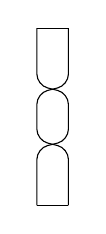
\begin{tikzpicture}[baseline]
				\node(xl1) at (-0.2,1){};
				\node(xr1) at (0.2,1){};	
				\node(xl2) at (-0.2, -1){};
				\node(xr2) at (0.2, -1){};
				\draw[rounded corners](xl1.north) to (-0.2,0.4) to (0.2, 0.3) to (0.2, -0.3) to (-0.2, -0.4) to (xl2.south);	
       				\draw[rounded corners](xr1.north) to (0.2,0.4) to (-0.2, 0.3) to (-0.2, -0.3) to (0.2, -0.4) to (xr2.south);
				\draw(xl1.north) to (xr1.north);
				\draw(xl2.south) to (xr2.south);	
			\end{tikzpicture} \\
			$b$ & & $t$ 
\end{tabular} \end{center}
This operad $RB$ is also clearly an action operad, since we can just define $\pi^{RB} : RB_n \to \mathrm{S}_n$ to act like $\pi^B$ on any braids, at which point the fact that $\pi(t) \in S_1 = \{e_1\}$ will automatically take care of the twists. To learn more about the ribbon braids and their operads, see Natalie Wahl's thesis \cite{ribbon1} on the subject, or her subsequent paper with Paolo Salvatore \cite{ribbon2}.

\begin{lem} \label{G0abel} For any action operad $G$, the group $G(0)$ is abelian.  
\end{lem}
\begin{proof}
\end{proof}

\begin{defn} Sub action operads \end{defn}

The most important example of sub action operads are those of the symmetric operad, $\mathrm{S}$. This is because \cref{actop} itself makes explicit reference to the symmetric groups, and so every action operad will end up related to some sub-operad of $\mathrm{S}$:

\begin{defn} For an arbitrary action operad $G$ the images of the underlying permutation maps $\pi^G_n : G(n) \to \mathrm{S}_n$ naturally form an action operad $\mathrm{im}(\pi^G)$, where
\begin{itemize}
\item the sets of operations are the images of $G$'s sets of operations under the homomorphisms $\pi^G$:
\begin{eq*} \mathrm{im}(\pi^G)(n) \quad := \quad \mathrm{im}(\pi^G_n) \end{eq*}
\item the underlying permutation maps are the evident inclusions:
\begin{eq*} \pi^{\mathrm{im}(\pi^G)}_n \, : \, \mathrm{im}(\pi^G)(n) \hookrightarrow \mathrm{S}_n \end{eq*}
\item the operad multiplication is the appropriate restriction of the multiplication of $\mathrm{S}$:
\begin{eq*} \mu^{\mathrm{im}(\pi^G)}( \, g \, ; \, h_1, ..., h_n \, ) \quad := \quad \mu^{\mathrm{S}}( \, g \, ; \, h_1, ..., h_n \, ) \end{eq*}
\end{itemize}
Clearly this $\mathrm{im}(\pi^G)$ is a sub action operad of the symmetric operad $\mathrm{S}$, and we will call the \emph{underlying permutation operad} of $G$.
\end{defn} 

For example, consider the action operad $\mathrm{B}$ we just saw in \cref{braidop}. For a given $n$, the braid group $\mathrm{B}_n$ is generated by $n-1$ elementary braids. But the underlying permutations of these braids are just the $n-1$ adjacent transpositions which generate the symmetric group $\mathrm{S}_n$, and so the underlying permutation maps $\pi^{\mathrm{B}}_n : \mathrm{B}_n \to \mathrm{S}_n$ are all surjective. Thus the underlying permutation operad of $\mathrm{B}$ is just the whole symmetric action operad $\mathrm{S}$.

It is even easier to see that $\mathrm{S}$ itself will have underlying permutations $\mathrm{S}$, as the maps $\pi^{\mathrm{S}}_n = \mathrm{id} : \mathrm{S}_n \to \mathrm{S}_n$ are obviously surjective. Similarly, the trivial operad $\mathrm{T}$ is also its own underlying permutation action operad, as the image of the homomorphims $\pi^{\mathrm{T}}_n : \{ e \} \to \mathrm{S}_n$ are trivial. Faced with rather dull examples like these, it might be tempting to try and construct some action operads with more exotic underlying permutations, like maybe the alternating groups $\mathrm{A}_n \subset \mathrm{S}_n$. But it turns out that this is not possible; when it come to their underlying permutation operad, action operads come in exactly two flavours.

\begin{defn} Let $G$ be an action operad where $\mathrm{im}(\pi)(n)$ is the trivial group for each $n \in \mathbb{N}$. Then we say that $G$ is \emph{non-crossed}, since its operad multiplication will be a true group homomorphism:
\begin{eq*} \begin{array}{rll}
			\mu( \, gg' \, ; \, h_1 h'_1, ..., h_n h'_n \, ) & = & \mu( \, g \, ; \, h_{\pi(g')^{-1}(1)}, ..., h_{\pi(g')^{-1}(n)} \, ) \mu( \, g' \, ; \, h'_1, ..., h'_n \, ) \\
			& = & \mu( \, g \, ; \, h_1, ..., h_n \, ) \mu( \, g' \, ; \, h'_1, ..., h'_n \, ) \\
		\end{array}
\end{eq*}
Likewise, a \emph{crossed} action operad will refer to any that has a non-trivial underlying permutation operad.
\end{defn}

\begin{lem}\label{surjortriv} An action operad $G$ is crossed if and only if it has surjective underlying permutation maps $\pi_n : G(n) \to \mathrm{S}_n$. In other words, the underlying permutations operad of $G$ must be either the trivial operad $\mathrm{T}$ or the symmetric operad $\mathrm{S}$.
\end{lem}
\begin{proof}
Let $\mathrm{im}(\pi)$ be the underlying permutation operad of $G$, and let us assume that $G$ is crossed, so that $\mathrm{im}(\pi)$ is not the trivial operad. This means that for some natural number $n$, the $n$-ary operations of $\mathrm{im}(\pi)$ include at least one permutation $\sigma$ which is not the identity element of the relevant symmetric group $\mathrm{S}_n$. Put another way, there must be some $\sigma$ and some $1 \le i \le n$ for which $\sigma(i) \neq i$. But now consider evaluating the expression
\begin{eq*} \mu^{\mathrm{im}(\pi)}( \, \sigma \, ; \, e_0, ..., e_0, e_1, e_0, ...., e_0, e_1, e_0, ..., e_0 \, ) \end{eq*}
where the $e_1$'s above are appearing in the $i$th and $\sigma(i)$th coordinates, which we know are distinct. From the definitions of $\mathrm{im}(\pi)(n)$ and of operad multiplication in $\mathrm{S}$, this permutation is really just
\begin{eq*} \mu^{\mathrm{S}}( \, \sigma \, ; \, e_0, ..., e_0, e_1, e_0, ...., e_0, e_1, e_0, ..., e_0 \, ) \quad = \quad (1 \, 2) \end{eq*}
the only non-identity element of $\mathrm{S}_2$. This proves that the map $\pi_2 : G(2) \to \mathrm{S}_2$ is indeed surjective, but more than that it shows that $\mathrm{im}(\pi)$ must contain every possible adjacent transposition, since for any $m \in \mathbb{N}$ we have
\begin{eq*} \begin{array}{rll}
			& & \mu^{\mathrm{im}(\pi)}( \, e_n \, ; \, e_1, ..., e_1, (1 \, 2), e_1, ...., e_1 \, ) \\
			& = & \mu^{\mathrm{S}}( \, e_n \, ; \, e_1, ..., e_1, (1 \, 2), e_1, ...., e_1 \, ) \\
			& = & (m \, \, m+1) \in \mathrm{S}_n
		\end{array}
\end{eq*}
Then because adjacent transpositions generate the symmetric groups $\mathrm{S}_n$, it follows that every permutation is actually an operation in $\mathrm{im}(\pi)$, so that it is really just the full symmetric operad $\mathrm{S}$. Thus by only assuming that our action operad $G$ was crossed, we have shown that all of the maps $\pi_n$ must be surjective.
\end{proof} 

\begin{defn} $G$-operads \end{defn}

\section{Operad algebras}

\begin{defn} Operad algbras \end{defn}

\begin{defn} $G$-operad algebras \end{defn}

\section{$\mathrm{E}G$-algebras}

\begin{defn} The $G$-operad $\mathrm{E}G$ \end{defn}

\begin{defn}\label{monaddef} The monad $\mathrm{E}G$ \end{defn}

\begin{defn} $\mathrm{E}G$-algebras \end{defn}

\begin{prop} $G$-operad algebras are monoidal categories with permutation-like structure \end{prop} 

\begin{cor} Braided monoidal categories are $G$-operad algebras \end{cor}

\begin{defn} A strict monoidal category $X$ is said to be \emph{spacial} if, for any object $x \in \mathrm{Ob}(X)$ and any endomorphism of the unit object $f: I \to I$, 
\begin{eq*} f \otimes \mathrm{id}_x = \mathrm{id}_x \otimes f \end{eq*}
\end{defn}

The motivation for the name `spacial' comes from the context of string diagrams \cite{graphicalmon}. In a string diagram, the act of tensoring two strings together is represented by placing those strings side by side. Since the defining feature of the unit object is that tensoring it with other objects should have no effect, the unit object is therefore represented diagrammatically by the absense of a string. An endomorphism of the unit thus appears as an entity with no input or output strings, detached from the rest of the diagram. In a real-world version of these diagrams, made out of physical strings arranged in real space, we could use this detachedness to grab these endomorphisms and slide them over or under any strings we please, without affecting anything else in the diagram. This ability is embodied algebraically by the equation above, and hence categories which obey it are called `spacial'.

\begin{lem}\label{spacial} If $G$ is a crossed action operad, then all $\mathrm{E}G$-algebras are spacial. \end{lem}
\begin{proof}
Let $G$ be a crossed action operad, let $X$ be a $\mathrm{E}G$-algebra, and fix $x \in \mathrm{Ob}(X)$ and \( f: I \to I \). From \cref{surjortriv} we know that \( \pi : G(2) \to S_2 \) is surjective, so that the set $\pi^{-1}( \, (1 \, 2) \, )$ is non-empty, and from the rules for composition of action morphisms we see that for any such $g \in \pi^{-1}( \, (1 \, 2) \, )$,
\begin{eq*}\begin{array}{rll}
		\alpha( \, g \, ; \, \mathrm{id}_x, \, \mathrm{id}_I \, ) \circ \alpha( \, e_2 \, ; \, \mathrm{id}_x, \, f \, ) & = & \alpha( \, g \, ; \, \mathrm{id}_x, \, f \, ) \\
		& = & \alpha( \, e_2 \, ; \, f, \, \mathrm{id}_x \, ) \circ \alpha( \, g \, ; \, \mathrm{id}_x, \, \mathrm{id}_I \, ) \\
		\end{array}
\end{eq*}
Thus in order to obtain the result we're after, it will suffice to find a particular $g \in \pi^{-1}( \, (1 \, 2) \, )$ for which
\begin{eq*}\alpha( \, g \, ; \, \mathrm{id}_x, \, \mathrm{id}_I \, ) = \mathrm{id}_x \end{eq*}
However, since
\begin{eq*}\begin{array}{rll}
		\alpha( \, g \, ; \, \mathrm{id}_x, \, \mathrm{id}_I \, ) & = & \alpha( \, g \, ; \, \mathrm{id}_x, \, \alpha( e_0; - ) \, ) \\
		& = & \alpha( \, \mu(g; e_1, e_0) \, ; \, \mathrm{id}_x \, )
		\end{array}
\end{eq*}
all we really need is to find a $g \in \pi^{-1}( \, (1 \, 2) \, )$ for which
\begin{eq*} \mu(g; e_1, e_0) = e_1 \end{eq*}
To this end, choose an arbitrary element $h \in \pi^{-1}( \, (1 \, 2) \, )$. This $h$ probably won't obey the above equation, but we can use it to construct a new element $g$ which does. Specifically, define
\begin{eq*} k \, := \, \mu( \, h \ ; \, e_1, \, e_0 \, ) \end{eq*}
and then consider
\begin{eq*} g \, := \, h \cdot \mu(e_2; k^{-1}, e_1) \end{eq*} 
To see that this is the correct choice of $g$, first note that we must have \( \pi(k) = e_1 \), since this is the only element of $S_1$. Following from that, we have 
\begin{eq*}\begin{array}{rll}
		\pi \big( \, \mu(e_2; k^{-1}, e_1) \, \big) & = & \mu \big( \, \pi(e_2) \ ; \, \pi(k^{-1}), \, \pi(e_1) \, \big) \\
		& = & \mu \big( \, e_2  \ ; \, e_1, \, e_1 \, \big) \\
		& = & e_2
		\end{array}
\end{eq*}
and hence
\begin{eq*}\begin{array}{rll}
		\pi(g) & = & \pi \big( h \cdot \mu(e_2; k^{-1}, e_1) \big) \\
		& = & \pi(h) \cdot \pi \big(\mu(e_2; k^{-1}, e_1) \big) \\
		& = & (1 \, 2) \cdot e_2 \\
		& = & (1 \, 2)
		.\end{array}
\end{eq*}
So $g$ is indeed in $\pi^{-1}( \, (1 \, 2) \, )$, and furthermore
\begin{eq*}\begin{array}{rll}
		\mu(g; e_1, e_0) & = & \mu \big( \, h \cdot \mu(e_2; k^{-1}, e_1) \ ; \, e_1, \, e_0 \, \big) \\
		& = & \mu( \, h \ ; \, e_1, \, e_0 \, ) \cdot \mu \big( \, \mu(e_2; k^{-1}, e_1) \ ; \, e_1, \, e_0 \, \big) \\
		& = & \mu( \, h \ ; \, e_1, \, e_0 \, ) \cdot \mu \big( \, e_2 \ ; \, \mu(k^{-1}; e_1), \, \mu(e_1; e_0) \, \big) \\
		& = & \mu( \, h \ ; \, e_1, \, e_0 \, ) \cdot \mu( \, e_2 \ ; \, k^{-1}, e_0 \, ) \\
		& = & k \cdot k^{-1} \\
		& = & e_1
		\end{array}
\end{eq*}
Therefore, $h \cdot \mu(e_2; k^{-1}, e_1)$ is exactly the $g$ we were looking for, and so working backwards through the proof we obtain the required result:
\begin{eq*} \begin{array}{rll}
		\mu(g; e_1, e_0) & = & e_1 \\
		\implies \quad \alpha( \, g \, ; \, \mathrm{id}_x, \, \mathrm{id}_I \, ) & = & \mathrm{id}_x \\
		& & \\
		\alpha( \, g \, ; \, \mathrm{id}_x, \, \mathrm{id}_I \, ) \circ \alpha( \, e_2 \, ; \, \mathrm{id}_x, \, f \, ) & = & \alpha( \, e_2 \, ; \, f, \, \mathrm{id}_x \, ) \circ \alpha( \, g \, ; \, \mathrm{id}_x, \, \mathrm{id}_I \, ) \\
		\implies \quad \alpha( \, e_2 \, ; \, \mathrm{id}_x, \, f \, ) & = & \alpha( \, e_2 \, ; \, f, \, \mathrm{id}_I \, )
		\end{array}
\end{eq*}
\end{proof}

\section{The free $\mathrm{E}G$-algebra on $n$ objects} 

Our goal for the next few chapters will be to understand the free braided monoidal category on an finite number of invertible objects. Thus, now that we have a firm grasp on action operads and their algebras, we should begin to think about the simpler free constructions they can form. We will use this extensively when calculating the invertible case later on. 

In the paper \cite{operadborel}, Gurski establishes how to contruct free $G$-operad algebras through the use of the monad $\mathrm{E}G$. What follows in this section is a quick summary of the results which will be useful for our purposes. For a more detailed treatment please refer to \cite{operadborel}.

\begin{prop}\label{freealg} There exists a free $\mathrm{E}G$-algebra on $n$ objects. That is, there is an $\mathrm{E}G$-algebra $Y$ such that for any other $\mathrm{E}G$-algebra $X$, we have an isomorphism of categories
\begin{eq*} \mathrm{E}G\mathrm{Alg}_S(Y, X) \cong X^n \end{eq*}
\end{prop}
\begin{proof}
There is an obvious forgetful 2-functor \( U: \mathrm{E}G\mathrm{Alg}_S \to \mathrm{Cat}\) sending $\mathrm{E}G$-algebras to their underlying categories. $U$ has a left adjoint, which we call the free 2-functor \( F : \mathrm{Cat} \to \mathrm{E}G\mathrm{Alg}_S \) adjoint to it. It follows immediately that
\begin{eq*}\begin{array}{rll}
		U(X)^n & = & \mathrm{Cat}(\{z_1, ..., z_n\}, U(X) ) \\
		& \cong & \mathrm{E}G\mathrm{Alg}_S( F(\{z_1, ..., z_n\}), X) 
		\end{array}
\end{eq*}
where $\{z_1, ..., z_n\}$ is any set with $n$ distinct elements. Since $X$ and $U(X)$ are obviously isomorphic as categories, this shows that $F(\{z_1, ..., z_n\})$ is the free algebra on $n$ objects as required. 
\end{proof}

\begin{defn}\label{Gndef} Let $\{ z_1, ..., z_n \}$ be an $n$-object set, which we will also consider as a discrete category. Then we will denote by $\mathbb{G}_n$ the $\mathrm{E}G$-algebra whose underlying category is $\mathrm{E}G( \{ z_1, ..., z_n \})$ and whose action
\begin{eq*} \alpha : \mathrm{E}G\big( \, \mathrm{E}G( \{ z_1, ..., z_n \}) \, \big) \to \mathrm{E}G( \{ z_1, ..., z_n \}) \end{eq*}
is the appropriate component of the multiplication natural transformation $\mu: \mathrm{E}G \circ \mathrm{E}G \to \mathrm{E}G$ of the 2-monad $\mathrm{E}G$.
\end{defn}

\begin{thm} $\mathbb{G}_n$ is the free $\mathrm{E}G$-algebra on $n$ objects. That is,
\begin{eq*}  F(\{z_1, ..., z_n\}) = \mathbb{G}_n \end{eq*}
\end{thm}
\begin{proof}
\end{proof}

\cref{Gndef} is a fairly opaque definition, so we'll spend a little time upacking it. Recall from \cref{monaddef} that $\mathrm{E}G( \{ z_1, ..., z_n \})$ is the coequalizer of the maps
\begin{eq*} \begin{tikzcd}
\coprod_{m \geq 0} \mathrm{E}G(m) \times G(m) \times \{ z_1, ..., z_n \}^m \ar[r, shift left] \ar[r, shift right] & \coprod_{m \geq 0} \mathrm{E}G(m) \times \{ z_1, ..., z_n \}^m
\end{tikzcd} \end{eq*}
that comes from the action of $G(m)$ on $\mathrm{E}G(m)$ by multiplication on the right,
\begin{eq*} \begin{array}{rll}
		\mathrm{E}G(m) \times G(m) & \to & \mathrm{E}G(m) \\
		(g, h) & \mapsto & gh \\
		( \, !: g \to g', \mathrm{id}_h \, ) & \mapsto & !: gh \to g'h
		\end{array}
\end{eq*}
and the action of $G(m)$ on $\{ z_1, ..., z_n \}^m$ by permutation,
\begin{eq*} \begin{array}{rll}
		G(m) \times \{ z_1, ..., z_n \}^m & \to & \{ z_1, ..., z_n \}^m \\
		( \, h \, ; \, x_1, ..., x_m \, ) & \mapsto & (x_{\pi(h^{-1})(1)}, ..., x_{\pi(h^{-1})(m)}) \\
		 \, (\mathrm{id}_h \, ; \, \mathrm{id}_{(x_1, ..., x_m)} \, ) & \mapsto & \mathrm{id}_{(x_{\pi(h^{-1})(1)}, ..., x_{\pi(h^{-1})(m)})}
		\end{array}
\end{eq*}

First, objects in this algebra are equivalence classes of tuples $(g; x_1, ..., x_m)$, for $g \in G(m)$ and $x_i \in \{z_1, ..., z_n\}$, under the relation
\begin{eq*} ( \, gh \, ; \, x_1, \, ..., \, x_m \, ) \sim ( \, g \, ; \, x_{\pi(h)^{-1}(1)}, \, ..., \, x_{\pi(h)^{-1}(m)} \, )\end{eq*}
Notice that using this relation we can rewrite any object uniquely in the form $[e; x_1, ..., x_m]$ for some $m \in \mathbb{N}$ and $x_i \in \{z_1, ..., z_n\}$. This means that each equivalence class is just the tensor product $x_1 \otimes ... \otimes x_m$ in the underlying monoidal category of $\mathbb{G}_n$, for some unique sequence of generators. That is, we can view the objects of $\mathbb{G}_n$ as elements of the monoid freely generated by each of the $z_i$, or in other words:

\begin{lem} \label{Gnobj} $\mathrm{Ob}(\mathbb{G}_n)$ is the free monoid on $n$ generators, $\mathbb{N}^{\ast n}$, the free product of $n$ copies of $\mathbb{N}$. \end{lem}

Similarly, the morphisms of $\mathbb{G}_n$ are the maps
\begin{eq*} (! ; \mathrm{id}_{x_1}, ..., \mathrm{id}_{x_m}) : ( g ; x_1, ..., x_m ) \to ( g' ; x_1, ..., x_m )\end{eq*}
with $g, g' \in G(m)$ and $x_i \in \{z_1, ..., z_n \}$. Using the relation $\sim$ on objects we can rewrite each of these morphisms in the form
\begin{eq*} [h ; \mathrm{id}_{y_1},...,\mathrm{id}_{y_m}] \, : \, y_1 \otimes ... \otimes y_m \, \to \, y_{\pi(h^{-1})(1)} \otimes ... \otimes y_{\pi(h^{-1})(m)} \end{eq*}
where
\begin{eq*} h = g' g^{-1}, \quad \quad y_i = x_{\pi(g^{-1})(i)} \end{eq*}
 The $\mathrm{E}G$-action of $\mathbb{G}_n$ is permutation and tensor product, and the action on morphisms is given by
\begin{eq*} \alpha( \, g \, ; \, [h_1; \mathrm{id}_{x_1}, ..., \mathrm{id}_{x_{m_1}}], \, ..., \, [h_k; \mathrm{id}_{x_1}, ..., \mathrm{id}_{x_{m_k}}] \, ) = [ \, \mu(g;h_1, .., h_k) \, ; \, \mathrm{id}_{x_1}, \, ..., \, \mathrm{id}_{x_{m_k}} \, ] \end{eq*}
Notice that using tensor product notation the object $[e; x]$ is simply $x$, and so $[e; \mathrm{id}_x] = \mathrm{id}_{[e;x]}$ should be written as $\mathrm{id}_x$. Hence by the above $[g; \mathrm{id}_{x_1}, ..., \mathrm{id}_{x_m}]$ is really just $\alpha(g; \mathrm{id}_{x_1}, ..., \mathrm{id}_{x_m})$, and so we have the following:

\begin{lem} \label{Gnmapsaction} Every morphism of $\mathbb{G}_n$ can be expressed uniquely as an action morphism 
\begin{eq*} \alpha( \, g \, ; \, \mathrm{id}_{x_1}, ..., \mathrm{id}_{x_m} \, ) \, : \, x_1 \otimes ... \otimes x_m \, \to \, x_{\pi(g)^{-1}(1)} \otimes ... \otimes x_{\pi(g)^{-1}(m)} \end{eq*}
for some $g, g' \in G(m)$ and $x_i \in \{z_1, ..., z_n \}$. \end{lem}

As an immediate consequence of this, the source and target of a given morphism in $\mathbb{G}_n$ must be related to one another by some permutation of the form $\pi(g)$. In toher words, the connected components of $\mathbb{G}_n$ will depend upon the underlying permutation operad of $G$, in the following way:

\begin{prop}\label{Gnconcomp} Considered as a monoid under tensor product,
\begin{eq*} \pi_0(\mathbb{G}_n) \quad = \quad \begin{cases}
							\quad \mathbb{N}^n & \text{if $G$ is crossed} \\
							\quad \mathbb{N}^{\ast n} & \text{otherwise}
							\end{cases}
 \end{eq*} 
Also, the canonical homomorphism sending objects in $\mathbb{G}_n$ to their connected component,
\begin{eq*} [ \, \_ \, ] \, : \, \mathrm{Ob}(\mathbb{G}_n) \to \pi_0(\mathbb{G}_n) \end{eq*}
is the quotient map of abelianisation
\begin{eq*} \mathrm{ab} \, : \, \mathbb{N}^{*n} \to (\mathbb{N}^{*n})^{\mathrm{ab}} \, = \, \mathbb{N}^n \end{eq*}
when $G$ is crossed, and the identity map $\mathrm{id}_{\mathbb{N}^{*n}}$ otherwise.
\end{prop}
\begin{proof}
By \cref{Gnmapsaction}, all morphisms in $\mathbb{G}_n$ can be written uniquely as $\alpha(g; \mathrm{id}_{x_1}, ..., \mathrm{id}_{x_m})$, for some $g \in G(m)$ and $x_i \in \{z_1, ..., z_n \}$, the set of generators of $\mathbb{N}^{*n}$. Since maps of this form have source $x_1 \otimes ... \otimes x_m$ and target $x_{\pi(g^{-1})(1)} \otimes ... \otimes x_{\pi(g^{-1})(m)}$, we see that the only pairs of object which might have a morphism between them are those that can be expanded as tensor products that differ by some permutation. 

If our action operad $G$ is crossed, then for any two objects like this --- say source $x_1 \otimes ... \otimes x_m$ and target $x_{\sigma^{-1}(1)} \otimes ... \otimes x_{\sigma^{-1}(m)}$ for an arbitrary $\sigma \in \mathrm{S}_m$ --- we can always find a map $\alpha(g; \mathrm{id}_{x_1}, ..., \mathrm{id}_{x_m})$ between them, because by \cref{surjortriv} the underlying permutations maps $\pi_m: G(m) \to S_m$ are all surjective and so there must exist at least one $g$ with $\pi(g) = \sigma$. In particular, for any two generating objects $z_i$ and $z_j$of $\mathbb{G}_n$ there must exist at least morphism between $z_i \otimes z_j$ and $z_j \otimes z_i$, and therefore
\begin{eq*} [z_i] \otimes [z_j] \quad = \quad [z_i \otimes z_j] \quad = \quad [z_j \otimes z_i] \quad = \quad [z_j] \otimes [z_i] \end{eq*}
Thus the canonical map $[ \, \_ \, ] : \mathrm{Ob}(\mathbb{G}_n) \to \pi_0(\mathbb{G}_n)$ is the one that makes the free product of $\mathbb{N}^{*n}$ commutative, that is, the quotient map for the abelianisation $\mathrm{ab} : \mathbb{N}^{*n} \to (\mathbb{N}^{*n})^{\mathrm{ab}}$, and so $\pi_0(\mathbb{G}_n) = \mathbb{N}^n$.

Conversely, if $G$ is non-crossed then its underlying permutation operad $\mathrm{im}(\pi)$ is trivial, and so the only morphisms we have in $\mathbb{G}_n$ will be those of the form
\begin{eq*} \alpha( \, e_m \, ; \, \mathrm{id}_{x_1}, ..., \mathrm{id}_{x_m} \, ) \quad = \quad \mathrm{id}_{x_1} \otimes ... \otimes \mathrm{id}_{x_m} \quad = \quad \mathrm{id}_{x_1 \otimes ... \otimes x_m} \end{eq*}
Therefore the map $[ \, \_ \,]$ just sends each object to its identity morphism, and since that function is one-to-one and onto it follows that
\begin{eq*} \pi_0(\mathbb{G}_n) \quad = \quad \mathrm{Ob}(\mathbb{G}_n) \quad = \quad \mathbb{N}^{\ast n}, \quad \quad \quad \quad \quad [ \, \_ \,] \quad = \quad \mathrm{id}_{\mathbb{N}^{*n}} \end{eq*}
by \cref{Gnobj}.
\end{proof} 

Finally, \cref{Gnmapsaction} also gives us a complete description of how the morphisms of $\mathbb{G}_n$ interact under tensor product, though we need a little new terminology in order to express it properly.

\begin{defn} Let $G$ be an action operad. Then we will also the notation $G$ to denote the \emph{underlying monoid} of this action operad. This is the natural way to consider $G$ as a monoid, with its element set being all of its elements together, $\bigsqcup_m G(m)$, and with tensor product as its binary operation, $g \otimes h = \mu(e_2; g, h)$.

Also, note that this monoid comes equipped with a homomorphism $| \, \_ \, | : G \to \mathbb{N}$, sending each $g \in G$ to the natural number $m$ if and only if $g$ is an element of the group $G(m)$. We'll call this number $|g|$ the \emph{length} of $g$.
\end{defn}

\begin{defn}\label{lengthdef} Let $S$ be a set and $F(S)$ the free monoid on $S$, the monoid whose elements are strings of elements of $S$ and whose binary operation is concatenation. Then we will denote by
\begin{eq*} | \, \_ \, | : F(S) \to \mathbb{N} \end{eq*}
the monoid homomorphism defined by sending each element of $S \subseteq F(S)$ to 1, and therefore also each concatenation of $n$ elements of $S$ to the natural number $n$. Again, we will call $|x|$ the \emph{length} of $x \in F(S)$.
\end{defn}

\begin{lem} \label{Gnmor} The monoid of morphisms of the algebra $\mathbb{G}_n$ is
\begin{eq*} \mathrm{Mor}(\mathbb{G}_n) \, \cong \, G \times_{\mathbb{N}} \mathbb{N}^{\ast n} \end{eq*}
where this pullback is taken over the respective length homomorphisms,
\begin{eq*} \begin{tikzcd}
G \times_{\mathbb{N}} \mathbb{N}^{\ast n} \ar[dd, shift left=4] \ar[rr] \ar[ddrr, phantom, "\lrcorner", very near start, shift left] & & \mathbb{N}^{\ast n} \ar[dd, "| \, \_ \, |"] & \\
& & & \\
\quad \quad G \ar[rr, "| \, \_ \, |"] & & \mathbb{N} &
\end{tikzcd} \end{eq*}
using the fact that $\mathbb{N}^{\ast n}$ is the free monoid $F\big( \, \{z_1, ..., z_n\} \, \big)$.
\end{lem}
\begin{proof}
An element of $G \times_{\mathbb{N}} F\big( \, \{z_1, ..., z_n\} \, \big)$ is just an element $g \in G(m)$ for some $m$, together with an $m$-tuple of objects $(x_1, ..., x_m)$ from the set of generators $\{z_1, ..., z_n\}$. Thus the action on $\mathbb{G}_n$ defines an obvious function 
\begin{eq*} \begin{array}{rlrll}
			\alpha & : & G \times_{\mathbb{N}} F\big( \, \{z_1, ..., z_n\} \, \big) & \to & \mathrm{Mor}(\mathbb{G}_n) \\
			& : & (g;x_1, ..., x_m) & \mapsto & \alpha(g; \mathrm{id}_{x_1}, ..., \mathrm{id}_{x_m})
		\end{array}
\end{eq*}
But by \cref{Gnmapsaction}, each element of $\mathrm{Mor}(\mathbb{G}_n)$ can be expressed in the form $\alpha(g; \mathrm{id}_{x_1}, ..., \mathrm{id}_{x_m})$ for a unique collection $(g;x_1, ..., x_m)$, and so this function $\alpha$ is actually a bijection of sets. Furthermore, this function preserves tensor product, since
\begin{eq*} \begin{array}{rll}
			\alpha\big( \, (g;f_1, ..., f_m) \otimes (g';f'_1, ..., f'_m) \, \big) & = & \alpha( \, g \otimes g' \, ; \, f_1, ..., f_m, f'_1, ..., f'_m \, ) \\
			& = & \alpha( \, g \, ; \, f_1, ..., f_m \, ) \otimes \alpha( \, g' \, ; \, f'_1, ..., f'_m \, )
		\end{array}
\end{eq*}
and hence it is a monoid isomorphism, as required.
\end{proof}